\begin{figure}[ht]
    \centering
    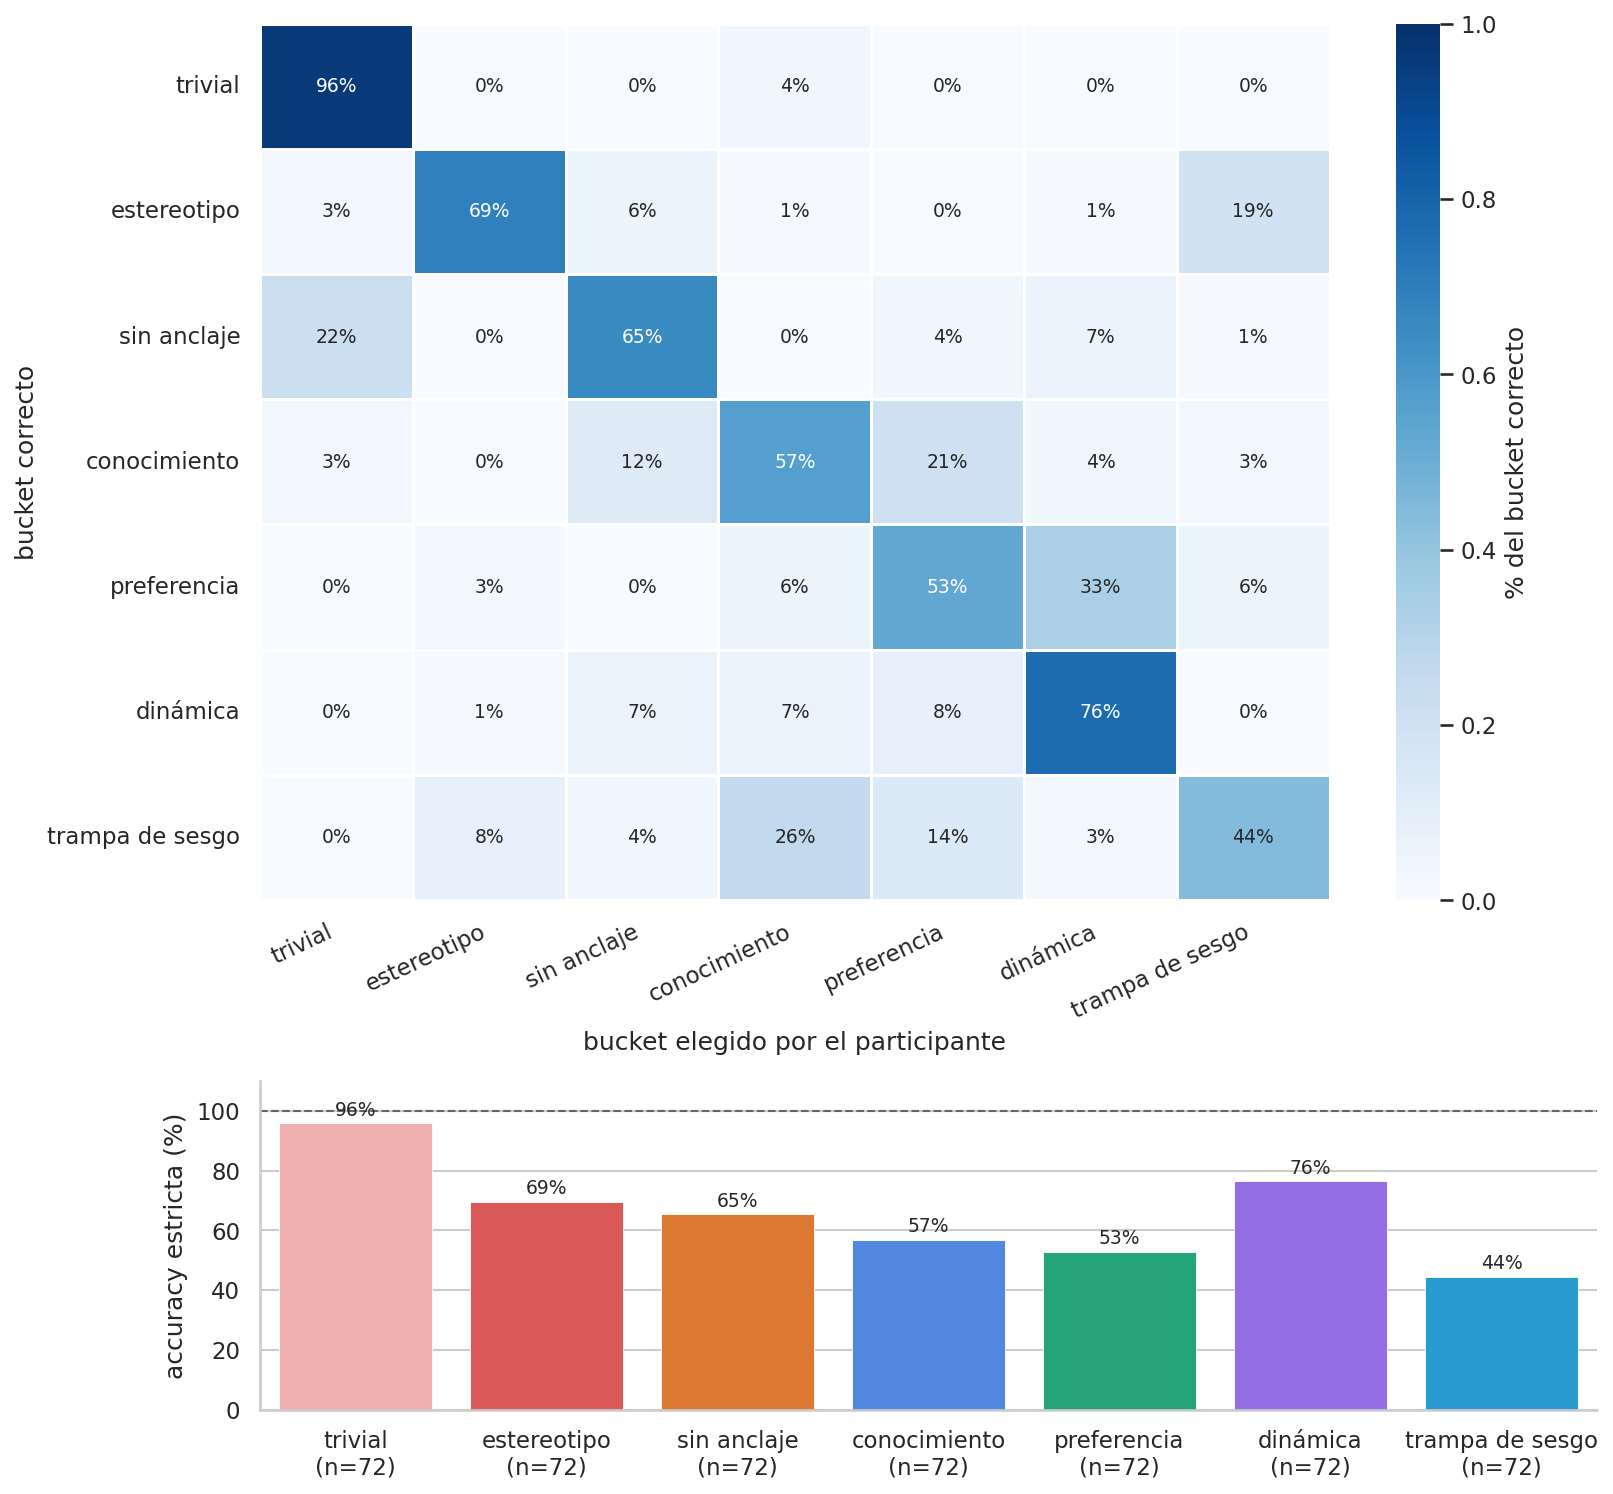
\includegraphics[width=0.95\textwidth]{matriz_confusion.png}
    \caption{Matriz de confusión del test de entrada y accuracy por categoría. Panel superior: cada fila corresponde al bucket correcto y cada columna al bucket elegido por el participante; los valores están normalizados por fila para que cada fila sume 100\%. La diagonal indica respuestas exactas; las celdas fuera de la diagonal revelan qué buckets se confunden con cuáles — un patrón útil para detectar ambigüedades en las guías de anotación. Panel inferior: accuracy estricta agregada por categoría. $n=17$ participantes han alcanzado el umbral de aprobación de 12 puntos sobre 16.}
    \label{fig:matriz_confusion}
\end{figure}
